\section{Auswertung}
\label{sec:Auswertung}
Der Eigenwiderstand des verwendeten Voltmeters beträgt $R_v=\SI{10}{\mega\ohm}$, dessen systematischer Fehler liegt bei $\num{+-1.5}\%$, der des Amperemeters beträgt $\num{+-3}\%$.
\subsection{Monozelle und Gegenspannung}
\label{ch:auswertung}
Der wie in der Durchführung beschriebene gemessene Wert für die Leerlaufspannung der Monozelle beträgt $U_{0,\text{mono}} = \SI{1.55}{\volt}$.
Bei der folgenden Messreihe wird der Widerstand $R_a$ jeweils in einem Bereich von $\SI{0}{\ohm}$ bis $\SI{50}{\ohm}$ variiert.
Die Messwerte sind in Tabelle \ref{tab:1} für die Monozelle und in Tabelle \ref{tab:2} für die Schaltung mit zusätzlicher Gegenspannung dargestellt.
\begin{table}
  \hspace*{\fill}
  \begin{subfigure}{0.40\textwidth}
  \centering
  \caption{Messdaten Monozelle.}
  \label{tab:1}
  \sisetup{table-format=3.4}
  \begin{tabular}{c c c}
    \toprule
    {$R_a-\text{Wert}$} & {$I [\si{\milli\ampere}]$} & {$U_k [\si{\volt}]$} \\
    \midrule
    \input{build/monotabelle.tex}
    \bottomrule
  \end{tabular}
\end{subfigure}
\hspace*{\fill}
\begin{subfigure}{0.40\textwidth}
  \centering
  \caption{Messdaten Gegenspannung.}
  \label{tab:2}
  \sisetup{table-format=3.4}
  \begin{tabular}{c c c}
    \toprule
    {$R_a-\text{Wert}$} & {$I [\si{\milli\ampere}]$} & {$U_k [\si{\volt}]$} \\
    \midrule
    \input{build/gegentabelle.tex}
    \bottomrule
  \end{tabular}
\end{subfigure}
\\
\hspace*{\fill}
\hspace*{\fill}
\caption{Messdaten für die Monozelle und die Gegenspannung.}
\end{table}

Somit ergibt sich der Monozellenplot in Abbildung \ref{fig:1},

\begin{figure}[H]
  \centering
  \includegraphics[height=8cm]{build/monoplot.pdf}
  \caption{Monozellenplot.}
  \label{fig:1}
\end{figure}

sowie der Plot mit der angesetzten Gegenspannung in Abbildung \ref{fig:2}

\begin{figure}[H]
  \centering
  \includegraphics[height=8cm]{build/gegenplot.pdf}
  \caption{Gegenspannungsplot.}
  \label{fig:2}
\end{figure}

Beide Ausgleichsgeraden werden mit SciPy auf eine lineare Funktion inklusive Fehlerbalken der Form
\begin{equation}
  f(x) = b + mx
  \label{eqn:mxb}
\end{equation}
gefittet, wobei für die Monozelle
\begin{equation}
  U_k(I) = U_0 - R_iI
    \label{eqn:uk}
\end{equation}
und für die gegenläufige Schaltung
\begin{equation}
  U_k(I) = U_0 + R_iI
\end{equation}
gilt.
Zur Berechnung der jeweiligen Leerspannung und des Innenwiderstandes wird die Methode der linearen Regression,
\begin{align}
  m &= \frac{ n \sum_{i=1}^n x_i y_i - \sum_{i=1}^n x_i \sum_{i=1}^n y_i }{n\sum_{i=1}^n x_i^2 - ( \sum_{i=1}^n x_i )^2}  \label{eqn:2}\\
  \notag\\
  b &= \frac{ \sum_{i=1}^n x_i^2 \cdot \sum_{i=1}^n y_i - \sum_{i=1}^n x_i \cdot \sum_{i=1}^n x_i y_i}{n\sum_{i=1}^n x_i^2 - ( \sum_{i=1}^n x_i )^2},
  \label{eqn:3}
\end{align}
bei $n$ Messwerten, gewählt.
\\
Die Standardabweichungen berechnen sich zu
\begin{align}
  \sigma_m &= \sqrt{ \sigma_y^2 \frac{n}{n \sum_{i=1}^n x_i^2 - (\sum_{i=1}^n x)^2} }
  \label{eqn:4}\\
  \notag\\
  \sigma_b &= \sqrt{ \sigma_y^2 \frac{\sum_{i=1}^n x_i^2}{n \sum_{i=1}^n x_i^2 - (\sum_{i=1}^n x)^2} }
  \label{eqn:5}
\end{align}
für die Steigung $m$, welche für den Innenwiderstand $R_i$ steht, und für den y-Achsenabschnitt $b$, der die Leerlaufspannung $U_0$ darstellt.\cite{fehler}
Daraus folgen die jeweiligen Werte
\begin{align*}
  U_{0,{\text{mono}}}  &= \input{build/mono_u0.tex}  & R_{i,\text{mono}}  &= \input{build/mono_ri.tex},\\
  U_{0,{\text{gegen}}} &= \input{build/gegen_u0.tex} & R_{i,\text{gegen}} &= \input{build/gegen_ri.tex}.
\end{align*}

Es ist zu erwähnen, dass bei der anfänglichen Messung der Leerlaufspannung der Monozelle durch den vorhandenen Innenwiderstand des Voltmeters ergibt.
Aus Gleichung \ref{eqn:klemmspannung} folgt, wenn der Eigenwiderstand des Voltmeters $R_v$ für $R_a$ eingesetzt wird sowie die aus der Maschenregel folgende Relation
\begin{equation}
  I = \frac{U_k}{R_v}
\end{equation}
genutzt wird, direkt die Formel
\begin{equation}
  U_0 = U_k + \frac{R_i}{R_v}U_k
\end{equation}
für die wahre Leerlaufspannung.
Mit den gegebenen Werten für $R_i$ und $R_v$ beträgt die Abweichung von $U_0$ zu $U_k$
\begin{align*}
  \increment{U_0} = \input{build/error_U0.tex}.
\end{align*}
Würde das Amperemeter in Abbildung \ref{fig:schaltung1} zwischen der Spannungsquelle und dem Voltmeter liegen, so würde der Innenwiderstand des Amperemeters ebenfalls einen zusätzlichen systematischen Fehler ergeben.
\subsection{Rechteckspannung und Sinusspannung}
Bei der Messung unter einer Rechteckspannung wird $R_a$ zwischen $\SI{20}{\ohm}$ bis $\SI{250}{\ohm}$ variiert, bei der Messung unter der Sinusspannung zwischen $\SI{100}{\ohm}$ bis $\SI{5000}{\ohm}$. \\
Die direkte Messung der Rechteckspannung am Generator ergibt $U_{0, \text{rechteck}} = \SI{0.56}{\volt}$, die direkte Messung der Sinusspannung ergibt $U_{0, \text{sinus}} = \SI{2}{\volt}$.
Es ergeben sich die in Tabelle \ref{tab:3} und Tabelle \ref{tab:4} angegebenen Messwerte.
\begin{table}[H]
  \hspace*{\fill}
  \begin{subfigure}{0.40\textwidth}
  \centering
  \caption{Messdaten Rechteckspannung.}
  \label{tab:3}
  \sisetup{table-format=3.4}
  \begin{tabular}{c c c}
    \toprule
    {$R_a-\text{Wert}$} & {$I [\si{\milli\ampere}]$} & {$U_k [\si{\volt}]$} \\
    \midrule
    \input{build/rechtecktabelle.tex}
    \bottomrule
  \end{tabular}
\end{subfigure}
\hspace*{\fill}
\begin{subfigure}{0.40\textwidth}
  \centering
  \caption{Messdaten Sinusspannung.}
  \label{tab:4}
  \sisetup{table-format=3.4}
  \begin{tabular}{c c c}
    \toprule
    {$R_a-\text{Wert}$} & {$I [\si{\milli\ampere}]$} & {$U_k [\si{\volt}]$} \\
    \midrule
    \input{build/sinustabelle.tex}
    \bottomrule
  \end{tabular}
\end{subfigure}
\\
\hspace*{\fill}
\hspace*{\fill}
\caption{Messdaten für die Rechteckspannung und Sinusspannung.}
\end{table}
Hieraus ergibt sich für die Messung der Rechteckspannung der in Abbildung \ref{fig:3} angegebene Plot, für die Messung der Sinusspannung der in Abbildung \ref{fig:4} angegebene Plot.
\begin{figure}[H]
  \centering
  \includegraphics[height=8cm]{build/rechteckplot.pdf}
  \caption{Rechteckspannungsplot.}
  \label{fig:3}
\end{figure}
\begin{figure}[H]
  \centering
  \includegraphics[height=8cm]{build/sinusplot.pdf}
  \caption{Sinusspannungsplot.}
  \label{fig:4}
\end{figure}
Analog zur Rechnung bei der Monozelle sowie bei der Gegenspannung werden mit SciPy Ausgleichsgeraden erstellt.
Dabei werden die Messwerte an die Funktion \ref{eqn:mxb} gefittet, so dass aus den errechneten Parametern nach \ref{eqn:uk} der Innenwiderstand $R_i$ und die Leerspannung $U_0$ abgelesen werden können.
Der y-Achsenabschnitt, die Steigung sowie deren Fehler berechnen sich nach (\ref{eqn:2}), (\ref{eqn:3}), (\ref{eqn:4}) und (\ref{eqn:5}), so dass sich die Werte
\begin{align*}
  U_{0,{\text{rechteck}}}  &= \input{build/rechteck_u0.tex},  & R_{i,\text{rechteck}}  &= \input{build/rechteck_ri.tex},\\
  U_{0,{\text{sinus}}} &= \input{build/sinus_u0.tex}, & R_{i,\text{sinus}} &= \input{build/sinus_ri.tex}
\end{align*}
ergeben

\subsection{Leistung im Belastungswiderstand}
Im Folgenden werden die Messergebnisse der Monozellenmessung aus Tabelle \ref{tab:1} betrachtet.
Aus der gemessenen Klemmspannung $U_k$ sowie dem Strom $I$ lässt sich die Leistung zu
\begin{equation}
  P = U_k I
\end{equation}
berechnen.
Diese Leistung wird gegen den Belastungswiderstand $R_a$ abgetragen, welcher sich aus
\begin{equation}
  R_a = \frac{U_k}{I}
\end{equation}
ergibt.
Hieraus folgen die in Tabelle \ref{tab:leistung} angegebenen Werte.

\begin{table}
  \centering
  \caption{Leistung in Abhängigkeit des Belastungswiderstandes.}
  \label{tab:leistung}
  \sisetup{table-format=3.4}
  \begin{tabular}{c c c c}
    \toprule
    {$R_a [\si{\ohm}]$} & {$\increment R_a [\si{\ohm}]$} & {$P [\si{\watt}]$} & {$\increment P [\si{\watt}]$} \\
    \midrule
    \input{build/P_tabelle.tex}
    \bottomrule
  \end{tabular}
\end{table}

Für die Fehlerrechnung der einzelnen Fehler wird bei der vorliegenden Rechnung und bei allen folgenden Rechnungen das Gaußsche Fehlerfortpflanzungsgesetz
\begin{equation}
\increment{f} = \sqrt{\Bigl(\frac{\partial f}{\partial x_1}\increment{x_1}\Bigr)^2 + \Bigl(\frac{\partial f}{\partial x_2}\increment{x_2}\Bigr)^2 + \dotsc + \Bigl(\frac{\partial f}{\partial x_n}\increment{x_n}\Bigr)^2}
\end{equation}
für eine Funktion $f(x_1,x_2, \dotsc ,x_n)$, bei der die Größen $x_1, x_2, \dotsc , x_n$ voneinander unabhängig sind, verwendet.
Hieraus folgt für den Fehler von $P$ die Fehlerformel
\begin{equation}
  \increment{P} = \sqrt{ \Bigl( I \increment{U_k} \Bigr)^2 + \Bigl( U_k \increment{I}  \Bigr)^2 }
\end{equation}
sowie für $R_a$ die Fehlerformel
\begin{equation}
  \increment{R_a} = \sqrt{ \Bigl( \frac{1}{I} \increment{U_k} \Bigr)^2 + \Bigl( - \frac{U_k}{I^2} \increment{I}  \Bigr)^2}.
\end{equation}
Zudem wird als Theoriekurve die Leistung nach Formel \ref{eqn:leistung} sowie nach Formel \ref{eqn:klemmspannung} zu
\begin{equation}
  P = \frac{U_0^2}{(R_i + R_a)^2} R_a
\end{equation}
bestimmt.
Hierbei werden für $R_i$ sowie $U_0$ die in Kapitel \ref{ch:auswertung} bestimmten Werte genutzt.
Es ergibt sich somit der in Abbildung \ref{fig:5} dargestellte Plot.
\\
\begin{figure}[H]
  \centering
  \includegraphics[height=8cm]{build/leistung.pdf}
  \caption{Leistung in Abhängigkeit des Belastungswiderstandes.}
  \label{fig:5}
\end{figure}
%\begin{figure}
%  \centering
%  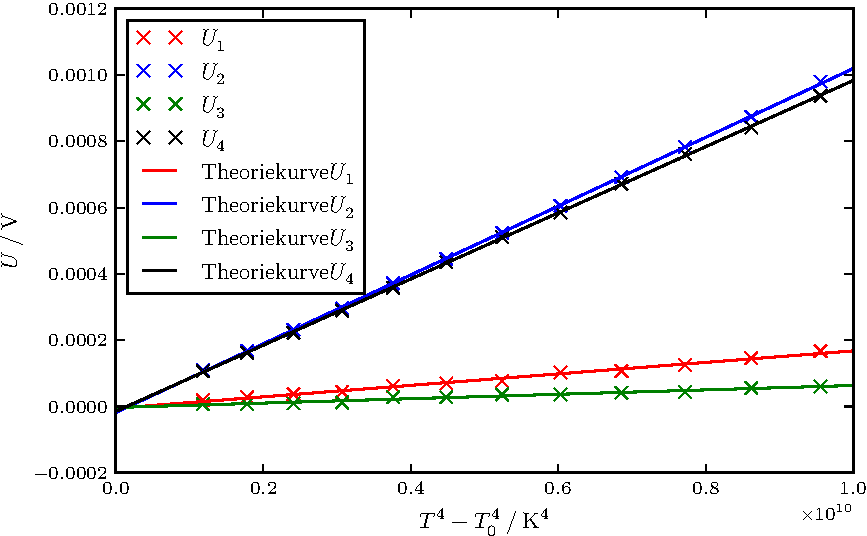
\includegraphics{plot.pdf}
%  \caption{Plot.}
%  \label{fig:plot}
%\end{figure}
%
%\begin{table}
%  \centering
%  \caption{Beispieltabelle}
%  \label{tab:tabelle_beispiel}
%  \sisetup{table-format=1.2}
%  \begin{tabular}{c c}
%    \toprule
%    {$a [\si{\second}]$} & {$b [\si{\kelvin}]$}\\
%    \midrule
%    1.0000  & 11.00 \\
2.0000  & 12.00 \\
3.0000  & 13.00 \\
4.0000  & 14.00 \\
5.0000  & 15.00 \\
6.0000  & 16.00 \\
7.0000  & 17.00 \\
8.0000  & 18.00 \\
9.0000  & 19.00 \\
10.0000 & 20.00 \\

%    \bottomrule
%  \end{tabular}
%\end{table}
%
%Es ergibt sich
%\begin{align}
%  a &= (0 \pm 0) ~ \si{\joule\per\kelvin\per\gram}
 \\
%\end{align}
